\documentclass{beamer}
\mode<presentation>
\usetheme{CambridgeUS}
\usepackage[russian]{babel}
\usepackage[utf8]{inputenc}
\usepackage[T2A]{fontenc}
\usepackage{sansmathaccent}

\usepackage{verbatim}
\usepackage{alltt}

\pdfmapfile{+sansmathaccent.map}
\title[Файловая система]{Операции над файлами в Linux}
\author{Наумов Д.А., доц. каф. КТ}
\date[12.11.2019] {Операционные системы и системное программное обеспечение, 2019}

\begin{document}

%ТИТУЛЬНЫЙ СЛАЙД
\begin{frame}
  \titlepage
\end{frame}
  
%СОДЕРЖАНИЕ ЛЕКЦИИ
\begin{frame}
  \frametitle{Содержание лекции}
  \tableofcontents  
\end{frame}

\section{Операции над файлами}

\subsection{Удаление файла}

\begin{frame}[fragile]{Удаление файла: unlink()}
Для удаления файла служит системный вызов unlink(), объявленный в заголовочном файле unistd.h следующим образом:
\begin{alltt}
int unlink (const char * FNAME);
\end{alltt}
\begin{itemize}
\item Аргумент FNAME — это имя удаляемого файла. 
\item unlink() возвращает 0 при успешном завершении. 
\item В случае ошибки возвращается –1.
\end{itemize}
\end{frame}

\begin{frame}[fragile]{Удаление файла: unlink()}
\begin{alltt}
#include <stdio.h>
#include <unistd.h>

int main (int argc, char ** argv)
\{
  if (argc < 2) return 1;
  
  if (unlink (argv[1]) == -1) \{
    fprintf (stderr, "Cannot unlink file (\%s)", argv[1]);
    return 1;
  \}
  
  return 0;
\}
\end{alltt}
\end{frame}

\begin{frame}
\begin{block}{Файл}
комплексное понятие, состоящее из следующих компонентов:
\begin{itemize}
\item данные (data);
\item индексы (inodes);
\item ссылки (links).
\end{itemize}
\end{block}
\begin{block}{Индексы}
специальные ячейки памяти, зарезервированные файловой системой для разделения данных на файлы. 
\end{block}
\begin{itemize}
\item Каждый индекс имеет уникальный (в рамках данной файловой системы) номер.
\item Индексы содержат информацию о том, в каких блоках файловой системы хранятся данные конкретного файла. 
\item В индексах содержатся сведения о дате и времени открытия и модификации файла. 
\item Сылка - имя индексного узла файловой системы. 
\end{itemize}
\end{frame}

%\section{Права доступа}

%\begin{figure}[h]
%\centering
%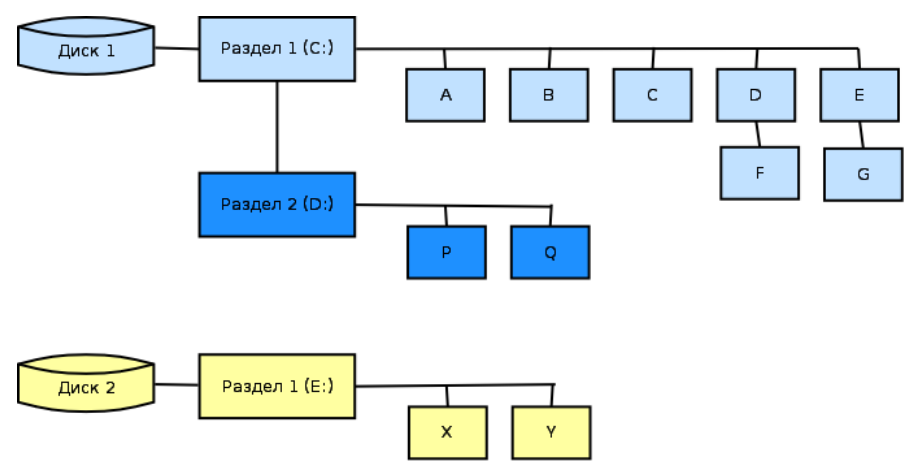
\includegraphics[scale=0.5]{images/lec09-pic01.png}
%\end{figure}

\end{document}